\documentclass[tikz,border=0pt]{standalone}
\usepackage{tikz}
\begin{document}
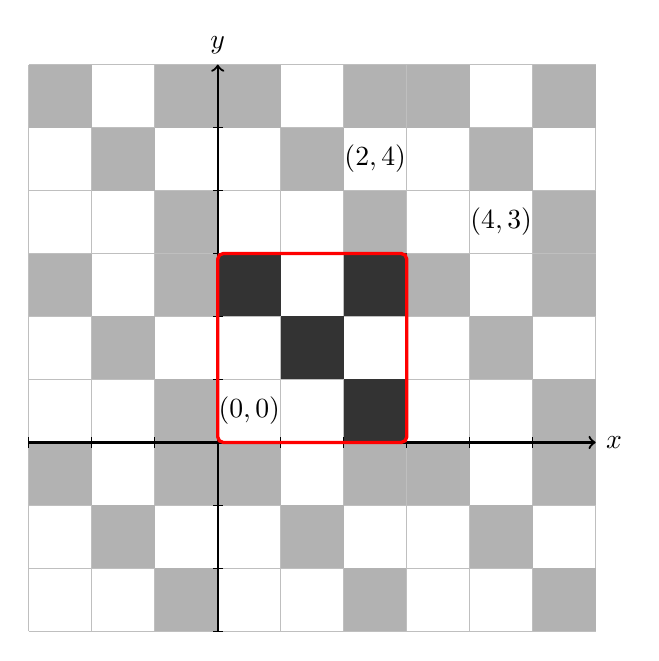
\begin{tikzpicture}[scale=0.8]

  \def\W{3}   % tile width (cols)
  \def\H{3}   % tile height (rows)
  % How many tiles to show in each direction
  \def\NX{2}
  \def\NY{2}

  \pgfmathsetmacro{\leftside}{-1}
  \pgfmathsetmacro{\rightside}{1}
  % Draw the tiled pattern
  \foreach \i in {\leftside,...,\rightside}{
    \foreach \j in {\leftside,...,\rightside}{
      \begin{scope}[shift={(\i*\W,\j*\H)}]
        % Draw grid lines
        \draw[thin,gray!50] (0,0) grid (\W,\H);

        % Repeat this pattern infinitely
        \fill[gray!60] (1,1) rectangle ++(1,1);
        \fill[gray!60] (2,0) rectangle ++(1,1);
        \fill[gray!60] (0,2) rectangle ++(1,1);
        \fill[gray!60] (2,2) rectangle ++(1,1);
      \end{scope}
    }
  }

  % Axes
  \draw[->,thick] (-\W*\NX+3,0) -- (\W*\NX,0) node[right] {$x$};
  \draw[->,thick] (0,-\H*\NY+3) -- (0,\H*\NY) node[above] {$y$};

  % Mark origin with (0,0)
  \fill (0.5,0.5) node {$(0,0)$};

  % Mark coordinates of first query
  \fill (2.5,4.5) node {$(2,4)$};
  \fill (4.5,3.5) node {$(4,3)$};
  
  % Integer ticks on axes
  \foreach \k in {4,-3,-2,-1,1,2,3,4,5}{
    \draw (\k,0.08) -- (\k,-0.08); % small x tick
    \draw (0.08,\k) -- (-0.08,\k); % small y tick
  }
  
  % Draw base tile as black
  \fill[black!80] (2,2) rectangle ++(1,1);
  \fill[black!80] (1,1) rectangle ++(1,1);
  \fill[black!80] (0,2) rectangle ++(1,1);
  \fill[black!80] (2,0) rectangle ++(1,1);

  % Highlight the base tile with red border
  \draw[red,very thick,rounded corners=2pt] (0,0) rectangle (\W,\H)
    node[midway,above right,xshift=2pt] {};

\end{tikzpicture}
\end{document}
